\documentclass[12pt]{article}
\usepackage{amsfonts,amssymb}
\usepackage{exercise}
\usepackage{amsmath}
\usepackage{amsthm}
\usepackage{hyperref}
\usepackage{graphicx}
\usepackage{listings}
%\documentstyle[12pt,amsfonts]{article}
%\documentstyle{article}

\setlength{\topmargin}{-.5in}
\setlength{\oddsidemargin}{0 in}
\setlength{\evensidemargin}{0 in}
\setlength{\textwidth}{6.5truein}
\setlength{\textheight}{8.5truein}
%
%\input ../adgeomcs/lamacb.tex
%\input ../mac.tex
%\input ../mathmac.tex
%
\input xy
\xyoption{all}
\def\fseq#1#2{(#1_{#2})_{#2\geq 1}}
\def\fsseq#1#2#3{(#1_{#3(#2)})_{#2\geq 1}}
\def\qleq{\sqsubseteq}
\newtheorem{theorem}{Theorem}
%cis51109hw1

%
\begin{document}
\begin{center}
\fbox{{\Large\bf Recursion and Big-O}}\\
\vspace{1cm}
\end{center}

\vspace{0.5cm}\noindent


\section*{Recursion}
The idea behind recursion is the same as that being used in proofs by induction. Can we show the fact that if a problem is solved (if a theorem is true) for smaller instances (for n-1, n-2 etc) then the problem is solvable (then the theorem is true) for the current instance (for n).

The canonical example used to introduce recursion in most CS classes is factorial. Factorial has this nice property that $factorial(n) = n \times factorial(n-1)$. So when you write the function recursively there is this level of trust that goes on that should not make you really question something along the lines of 'why should I believe factorial(n-1) will get computed correctly'. The correct way of thinking is to say let me assume factorial(n-1) is computed correctly. Can I do something with that?

\subsection*{Proving a program works!}

It is sometimes important to know if a program really works. And by this we do not mean, is there a syntax error or a logical flaw. We are asking the question that in a world where the idea that you have (CS calls those algorithms) gets perfectly translated into code (in some non crazy programming language), can you prove that your program will work regardless of the input provided to it.

Now the current best practice in the industry to do this proof is to write a bunch of unit tests. But does unit testing equate to a proof of correctness?

Unfortunately, math will just laugh at that notion. Unit testing just amounts to proof by example. Wouldn't it be better if you could say it works for everything. That turns out to be a universal statement.

\medskip

So for factorial this is what you want to prove

This program will compute factorial correctly regardless of input! 

How do you actually write a proof? You rely on the fact that induction is recursion!

Here's a sketch of the proof.

Base case - observe that when n=0 then the program returns 1 and that happens to be the same as 0!

Induction hypothesis - we assume that factorial works just fine for 0,1,2,...,n-1

Now for computing factorial of $n$, see that the program computes it as $n \times factorial(n-1)$. But we know by induction that we actually have $factorial(n-1) = (n-1)!$.

So the program is just computing $n \times (n-1)!$. But that is just $n!$.

\section*{How long does it take? aka Big - O}

As noted before, in most cases in the industry, you do not care about proving the correctness of your code (depends on the industry of course). But you do care about how much time your program is going to take!

While there are several ways of measuring time, the theoretical computer science methodology is to basically focus on the particular aspect of scalability. 

Take for instance the case of searching through an array of size $n$.

The way a CS person expresses the time taken for an algorithm is to say the algorithm is O(f(n)). For instance the search problem can easily be shown to be what is called $O(n)$ (once you know the definition of O). So you will say 

Searching in an unsorted array is an O of n operation. 

or 

Searching is a linear operation.

\textbf{Definition of big-O}: 

Let f and g be two functions defined on some subset of the real numbers. One writes
\begin{align*}
f(x)=O(g(x))\text{ as }x\to\infty\,
\end{align*}

if and only if there is a positive constant $C$ such that for all sufficiently large values of $x$, $f(x)$ is at most $C$ multiplied by the absolute value of $g(x)$. That is, $f(x) = O(g(x))$ if and only if there exists a positive real number $C$ and a real number $n_0$ such that

\begin{align*}
|f(x)| \le \; C |g(x)|\text{ for all }x \ge n_0.
\end{align*}

While the formal definition is needed for math, most CS people think of it in terms of this graph

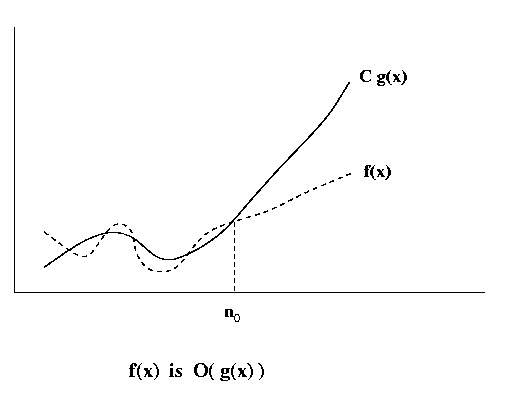
\includegraphics[scale=0.5]{./img/bigO.png}

Beyond a certain point, a constant multiple of one of the functions dominates the other.

\medskip

\textbf{Example}

Show that $n^2 + 100n$ is $O(n^2)$.

\medskip

Show in class why in this case you can set $C$ to be a number like 200 and $x_0$ to be $2$. Obviously other values are possible but the thing about the $O$ analysis is that you can be sloppy


\subsection*{Sloppiness is ok?}

Algorithmic complexity is interesting in that it deals with inequalities more than equalities. So you will often look at the expression for time taken and draw conclusions very quickly by dropping terms. For instance if you compute the relationship between search time and the size of the array and say that it is $100n$, that is actually generally expressed as $0(n)$. 

The constants do matter, but first it is important to make an efficient algorithm in the big - O sense. If you have two competing algorithms that are both linear, then you can worry about the constants. But if you have one which is linear and one which is quadratic, it should be clear which one is to be picked.

Therefore, remember that you are allowed to do some sloppy math when you are analyzing algorithms. The key is to begin the sloppiness only after you have written a correct expression down and done some level of evaluation.


\section*{Recurrences}

A recurrence relation in the most basic sense is an equation which is trying to define a sequence recursively.

So things like $f(n) = n * f(n-1)$ (factorial) or $T(n) = 2T(n/2) + n$ (merge sort recurrence). 

The analysis of algorithms that are recursive in nature boils down to solving recurrences and we will cover some theorems

\subsection*{First order Linear recurrences with constant coefficients}

\begin{theorem}
The closed form solution for
\begin{align*}
T(n) = \begin{cases}
rT(n-1) + g(n) & \mbox{if } n > 0\\
a & \mbox{if } n = 0
\end{cases}
\end{align*}

is given by

$T(n) = r^n a + \displaystyle\sum_{i=1}^n r^{n-i} g(i)$

\end{theorem}

\begin{proof}
The proof of most any property related to recursion and recurrences is best done with induction. 

Base case: When $n=0$, we have $T(0)= a$ as per the definition and as per the formula we have $r^0 a + \sum_{i=1}^0 r^{0-i}g(i)$. But the summation just returns 0 if we are going from a higher number to a lower number. So this just reduces to $r^0 a = a$.

Assume the formula is correct for $T(n-1)$.

We know $T(n) = rT(n-1) + g(n)$.

This is where the induction kicks in. Just substitute the formula for $T(n-1)$ since we have assumed that to be true.

\begin{align*}
T(n) = 
&r (r^{n-1} a + \sum_{i=1}^{n-1} r^{n-1-i} g(i)) + g(n) \\
&= r^n a + \sum_{i=1}^{n-1} r^{n-i} g(i) + g(n) \\
&= r^n a + \sum_{i=1}^{n-1} r^{n-i} g(i) + r^{n-n}g(n) \\
&= r^n a + \sum_{i=1}^{n} r^{n-i} g(i) 
\end{align*}

and this matches the claim being made for $T(n)$.

Combine this with the base case and we have a proof by induction.

\end{proof}

Application of the theorem.

This theorem can readily be applied for a whole number of `real world' problems.

For instance, here is a recursive way of finding the maximum element in an array

\begin{verbatim}
maximum(array) {
    if length(array) is 0 return n/a
    if length(array) is 1 return array[1]
    return max(firstelem,maximum(rest))
}
\end{verbatim}

How long does this function take? What is the running time of this algorithm? 

Both of these questions are generally meant to be answered in the big-O sense. In particular, we need to express $T(n)$ (the time taken on an input of size $n$) as $O(g(n))$ where $g(n)$ is one of the commonly found functions.

As we can see from the algorithm, to solve the $n$ sized version of the problem, we make one call to the function with an $n-1$ sized version of the problem and do a single computation after that.

\begin{align*}
T(n) = T(n-1) + 1
\end{align*}

and it is very easy to use the above theorem to see that the closed form solution for this recurrence is going to be $T(n) = n$. So the running time is $O(n)$.

\medskip

The Towers of Hanoi recursion works out to be $Moves(n) = 2Moves(n-1) + 1$. Also in this case we have $Moves(0) = 0$.

By direct application of the theorem we have the result that

\begin{align*}
Moves(n) &= 2^n \cdot 0+ \sum_{i=1}^n 2^{n-i} \cdot 1 \\
&=  2^{n-1} + 2^{n-2} + \ldots + 1 \\
&= 2^{n} - 1
\end{align*}

\subsection*{Binary search recurrence}

For mergesort we can write the recurrence as the following

\begin{align*}
T(n) = T(n/2) + T_{check}
\end{align*}

Also as a base case, assume that for an array of size 1, it takes constant time $a$. $T(1) = a$.

$T_{check}$ is the time taken to see whether the middle element is equal to the element that we are seeking. That should take the same amount of time as the base case. 

\begin{align*}
T(n) &= T(n/2) + a \\
&= T(n/4) + a + a \\
&= T(n/8) + a + a + a \\
&= T(n/2^i) + ia\\
&= a + a \log_2 n 
\end{align*}


which means that binary search is O( log n).

\end{document}



